In the context of eXplainable Artificial Intelligence
% , particularly for systems like $\text{LORE}_{sa}$, 
the visualization of high-dimensional data is of high relevance. When 
% $\text{LORE}_{sa}$ 
an explainability method
generates synthetic neighborhoods around the instance to be explained, the generated neighborhoods typically exist in a high-dimensional feature space that is difficult to interpret and visualize directly. Dimensionality reduction techniques serve as essential tools for projecting these multi-dimensional datasets into two or three-dimensional representations that enable human comprehension and interactive exploration \cite{yang2021dimensionality}.

The primary objective of dimensionality reduction in visual XAI is to preserve meaningful relationships and structures present in the original high-dimensional space while facilitating intuitive visual interpretation. 
% For $\text{LORE}_{sa}$'s, 
This capability is particularly crucial as it allows users to spatially explore the synthetic neighborhood and understand the distribution of generated instances. The choice of dimensionality reduction technique significantly impacts the quality of explanations. Different methods preserve distinct aspects of the data structure, while some excel at maintaining local neighborhoods, others are very good at preserving global relationships \cite{becht2019evaluation}.

% This challenge becomes more pronounced when dealing with the diverse nature of synthetic neighborhoods generated by $\text{LORE}_{sa}$'s genetic algorithms.
The effectiveness of different dimensionality reduction methods varies depending on the characteristics of the dataset, the size of the synthetic neighborhood, and the specific visual analytics requirements of the explanation task \cite{wang2021understanding}. The evaluation of dimensionality reduction techniques requires careful consideration of both local and global structure preservation criteria.

The following subsections examine four dimensionality reduction techniques. Each technique exhibits distinct characteristics in preserving data structure. We begin with \textbf{Principal Component Analysis (PCA)}, the most widely adopted linear method known for its computational efficiency and interpretability of component meanings. This is followed by \textbf{Multidimensional Scaling (MDS)}, a classical approach that focuses on preserving pairwise distances between data points. Subsequently, we explore \textbf{t-distributed Stochastic Neighbor Embedding (t-SNE)}, known for its effectiveness in revealing local cluster structures, though with limitations in global structure preservation. Finally, \textbf{Uniform Manifold Approximation and Projection (UMAP)}, which has shown superior performance in preserving both local and global structure while maintaining computational efficiency for large-scale synthetic neighborhoods.

The following subsections provide a detailed examination of each technique, followed by a comparative analysis that evaluates their relative performance across key criteria, including structure preservation, computational efficiency, and visual quality for neighborhood exploration. 

\subsubsection{PCA (Principal Component Analysis)}

Principal Component Analysis (PCA) represents one of the, if not the most, widely adopted linear dimensionality reduction technique in data analysis, with historical foundations dating back to the pioneering work of Pearson (1901) and Hotelling (1933) \cite{sewell2008pca}. As a fundamental method in multivariate statistics, PCA aims to reduce the dimensionality of datasets while preserving as much relevant information as possible through variance maximization \cite{sewell2008pca}.

% Source: Principal Component Analysis: A Natural Approach to Data Exploration, Page 70:3
\begin{figure}[htbp]
    \centering
    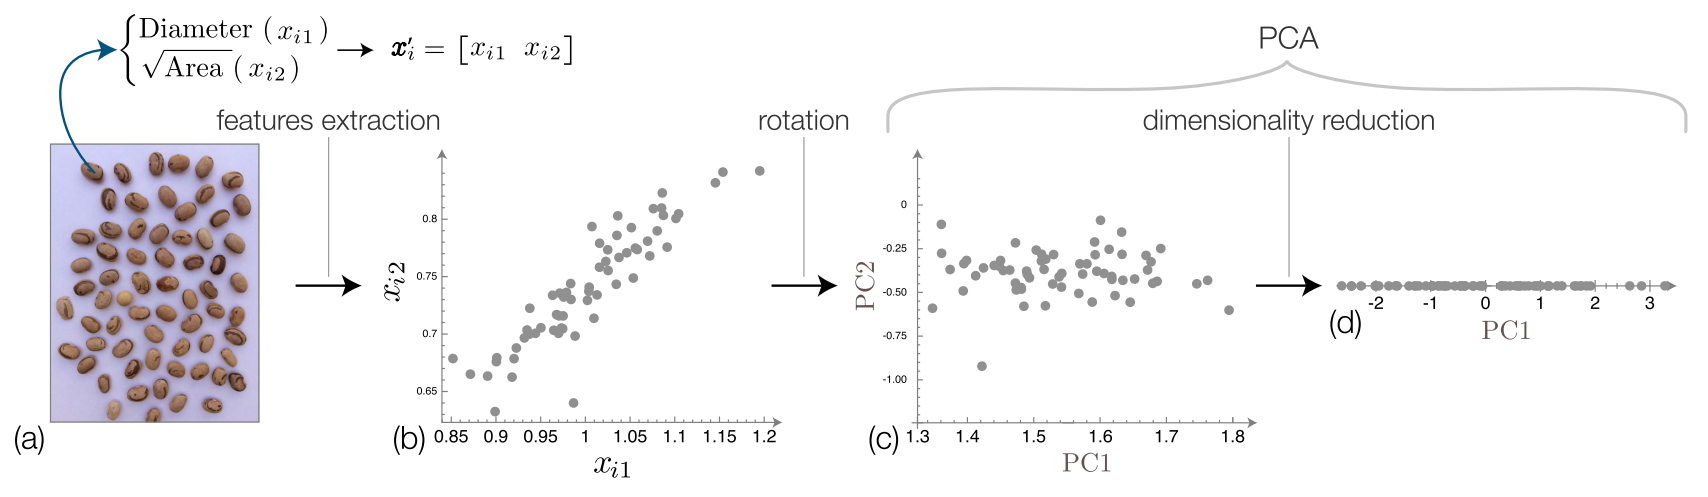
\includegraphics[width=1.0\textwidth]{images/PCA1.png}
    \caption{Illustration of the PCA process using real-world bean data. bean (a) is characterized in terms of two features: diameter xi1 and square root of area xi2. Though these two features are intrinsically related in a direct fashion,
bean shape variations induce a dispersion of the objects when mapped into the features space (b). PCA allows the identification of the orientation of maximum data dispersion (c). As the dispersion in the resulting
second axis is relatively small, this axis can be eventually disregarded (d).}
    \label{fig:pca_process}
\end{figure}

The theoretical foundation of PCA rests on the principles of linear transformation, where the algorithm transforms the data to a new coordinate system such that the new variables (principal components) are linear functions of the original variables, are not correlated, and are ordered by the amount of variance that they explain \cite{sewell2008pca}. The transformation operates as a rotation of the coordinate system that aligns the axes with the directions of maximum data variation \cite{gewers2021pca}, as illustrated in Figure~\ref{fig:pca_process}. This process can be expressed in matrix form as $Y = XW$, where $X$ represents the original data matrix, $W$ is the transformation matrix composed of eigenvectors, and $Y$ contains the principal component scores.

The algorithm's core mechanism involves computing the covariance matrix of the dataset, followed by eigenvalue decomposition to obtain eigenvectors and eigenvalues sorted in decreasing order \cite{sewell2008pca}. Each eigenvector defines the direction of a principal component, while the corresponding eigenvalue quantifies the amount of variance explained along that direction \cite{gewers2021pca}. An essential property of PCA is that the total data variance is preserved under the transformation: $\sum_{j=1}^{n} \sigma^2_{x_j} = \sum_{j=1}^{n} \sigma^2_{y_j}$, meaning the variance along each principal component equals the corresponding eigenvalue of the covariance matrix \cite{gewers2021pca}.

A distinctive characteristic of PCA is its ability to provide direct interpretability through loadings analysis. The transformation matrix $W$ contains eigenvectors that indicate how the original features contribute to each principal component, allowing users to understand which variables drive the main sources of variation in the data \cite{gewers2021pca}. 
PCA demonstrates particular effectiveness in scenarios involving correlated features, where the method can achieve substantial dimensionality reduction while retaining most of the original variance.
PCA's deterministic nature 
provides stability that is particularly valuable in interactive applications where consistent visualizations are required \cite{gewers2021pca}.

Particularly significant for 
eXplainable AI
% $\text{LORE}_{sa}$ 
applications is PCA's unique capability to preserve the structure of decision boundaries generated by the local surrogate models. Since PCA applies a linear transformation, the decision boundaries created by
% $\text{LORE}_{sa}$'s 
linear surrogate model maintain their essential geometric properties when projected into the two-dimensional visualization space. This preservation enables users to observe how the surrogate model rules translate into spatial regions within the spatial neighborhood analysis plot visualization, providing a direct correspondence between the rule-based explanations and the visual representation of the synthetic neighborhood. This characteristic distinguishes PCA from other dimensionality reduction techniques that may significantly distort or obscure the decision boundaries due to their nonlinear transformations.

However, PCA's linear assumption may limit its effectiveness for datasets with complex nonlinear structures. The algorithm's focus on variance maximization means that directions with high variance are prioritized regardless of their relevance for specific analytical tasks \cite{gewers2021pca}. 

\subsubsection{MDS (Multidimensional Scaling)}

Multidimensional Scaling (MDS) has theoretical origins tracing back to the pioneering work of Torgerson (1952) \cite{torgerson1952mds} in developing systematic methods for scaling multidimensional psychological and perceptual data. 

The core principle underlying MDS involves the preservation of pairwise distances between data points across different dimensional representations \cite{torgerson1952mds, mcinnes2020umap}. The algorithm operates by constructing a low-dimensional embedding where the Euclidean distances between points in the reduced space approximate as closely as possible the original distances (or dissimilarities) measured in the high-dimensional space. This distance-preserving objective distinguishes MDS from techniques that focus primarily on local neighborhood relationships or topological structures.

Classical MDS, also known as Principal \textbf{Coordinate} Analysis, employs a three-step procedure as originally formulated by Torgerson \cite{torgerson1952mds}.
The first step involves obtaining a scale of comparative distances between all pairs of stimuli (any set of objects, items, concepts, or entities in study), analogous to paired comparison methods but applied to distance relationships rather than direct stimulus comparisons. The second step requires estimating an additive constant to convert these comparative distances into absolute distances, addressing the inherent indeterminacy in the zero point of the distance scale. The third step determines the dimensionality of the space necessary to account for these absolute distances and computes the projections of data points onto the axes of this space.

MDS demonstrates particular strength in preserving global structure and long-range distance relationships within data \cite{mcinnes2020umap}. The algorithm's explicit focus on maintaining the full distance matrix makes it especially suitable for applications where all scales of structure are equally important, and where the preservation of metric relationships takes precedence over local neighborhood fidelity. This global perspective allows MDS to maintain meaningful relative positions between widely separated clusters or groups within the data.

The technique has robust theoretical properties from its foundation in classical metric geometry. Since MDS minimizes the sum of squared errors between original and embedded distances, it provides a principled approach to dimensionality reduction with well-understood optimality properties. The linear nature of classical MDS ensures deterministic results and computational stability, avoiding the convergence issues that can affect iterative nonlinear methods.

However, MDS faces several inherent limitations that constrain its effectiveness in specific visualization contexts. The algorithm's emphasis on preserving large pairwise distances can come at the expense of local neighborhood structure, potentially causing nearby points in the original space to appear more separated in the reduced dimensional representation than would be ideal for cluster identification \cite{maaten2008tsne}. This focus on global distance preservation means that MDS may not effectively capture local manifold structure or fine-grained clustering patterns that are crucial for understanding local decision boundaries in eXplainable AI applications.

Empirical evaluations on transcriptomic datasets reveal that MDS exhibits moderate performance in neighborhood preservation, 
indicating that local neighborhood relationships are less well preserved compared to methods specifically designed for local structure preservation \cite{yang2021dimensionality}. 
% In terms of computational efficiency, MDS shows the slowest runtime performance among the major dimensionality reduction techniques, particularly for larger datasets.

The algorithm's linear transformation approach means that MDS may struggle with datasets containing complex nonlinear manifold structures. While this linearity provides interpretability advantages similar to PCA, it can result in poor representations for data that lies on curved or twisted manifolds where Euclidean distances in the original space do not accurately reflect the intrinsic geometric relationships.

Despite these limitations, MDS offers several advantages for specific analytical contexts. The method's deterministic nature ensures reproducible results, which can be valuable for comparative analyses and scientific reporting. The explicit distance preservation objective makes MDS particularly suitable for applications where the maintenance of quantitative distance relationships is more important than the visual separation of clusters or local neighborhoods.

For 
% $\text{LORE}_{sa}$ 
synthetic neighborhoods visualization applications, MDS presents a mixed proposition. While the algorithm's distance preservation properties might maintain some aspects of the original synthetic neighborhood structure, its tendency to emphasize global relationships over local patterns may not optimally support the identification of 
local explanation regions that are central to 
% $\text{LORE}_{sa}$'s
eXplainable AI systems
interpretability objectives. 
Modern variants of MDS, including metric and non-metric forms, have been developed to address some of these limitations, but the classical formulation remains the most commonly implemented 
approach. 

\subsubsection{t-SNE (t-distributed Stochastic Neighbor Embedding)}

t-distributed Stochastic Neighbor Embedding (t-SNE) represents a nonlinear dimensionality reduction technique designed for data visualization \cite{maaten2008tsne}. Developed as an improvement over Stochastic Neighbor Embedding (SNE), t-SNE addresses fundamental challenges in high-dimensional data visualization by employing probabilistic modeling of pairwise similarities and takes advantage of heavy-tailed distributions to overcome the crowding problem in dimension reduction \cite{maaten2008tsne}.

\begin{figure}
    \centering
    \begin{subfigure}{0.45\textwidth}
        \centering
        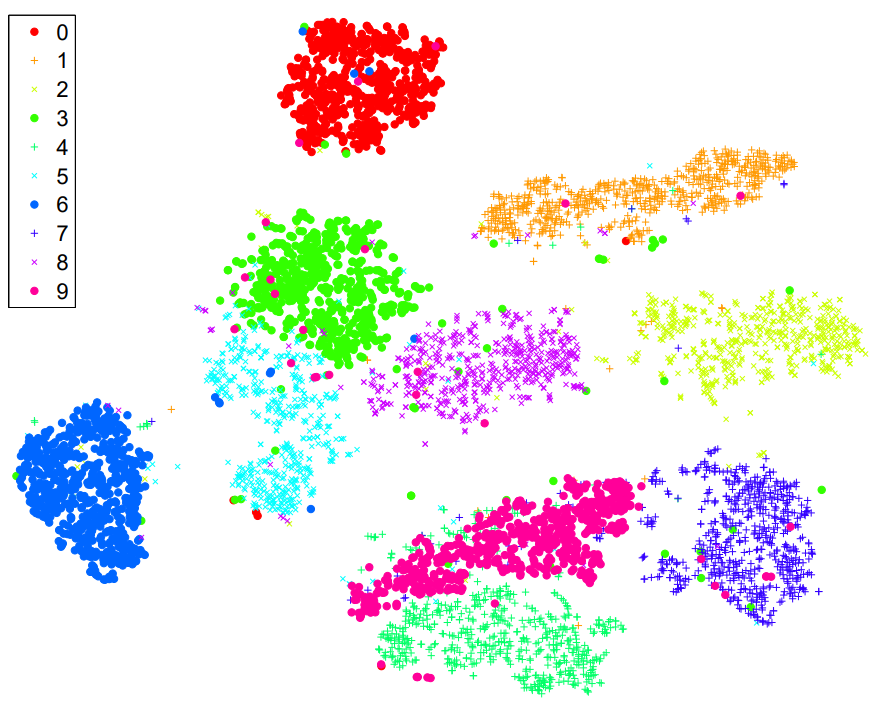
\includegraphics[width=\linewidth]{images/t-sne1.png}
        \caption{Visualization by t-SNE.}
        \label{fig:tsne_mnist_basic_tsne}
    \end{subfigure}
    \hfill
    \begin{subfigure}{0.45\textwidth}
        \centering
        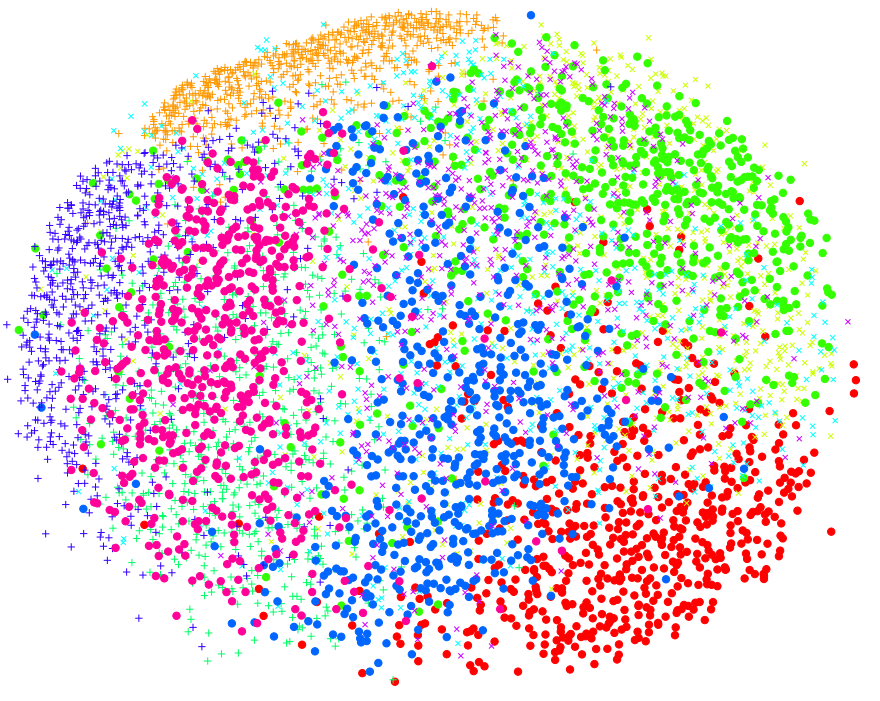
\includegraphics[width=\linewidth]{images/t-sne2.png}
        \caption{Visualization by Sammon mapping.}
        \label{fig:tsne_mnist_basic_sammon}
    \end{subfigure}
    \caption{Comparative visualization of 6,000 handwritten digits from the MNIST dataset using t-SNE (left) and Sammon mapping (right). The t-SNE visualization demonstrates superior cluster separation with clearly distinguishable digit groups (0-9), while Sammon mapping shows significant overlap between different digit classes. This comparison illustrates t-SNE's exceptional capability in preserving local neighborhood structures and creating meaningful cluster formations.}
    \label{fig:tsne_mnist_basic}
\end{figure}

The algorithmic foundation of t-SNE rests on converting high-dimensional Euclidean distances between data points into conditional probabilities that represent similarities. For each data point $x_i$, the algorithm defines the conditional probability $p_{j|i}$ that $x_i$ would select $x_j$ as its neighbor if neighbors were chosen proportionally to their probability density under a Gaussian centered at $x_i$ \cite{maaten2008tsne}. This probability is computed as $p_{j|i} = \frac{\exp(-\|x_i - x_j\|^2/2\sigma_i^2)}{\sum_{k \neq i} \exp(-\|x_i - x_k\|^2/2\sigma_i^2)}$, where $\sigma_i$ represents the variance of the Gaussian kernel around point $x_i$, determined by the perplexity parameter that controls the effective number of nearest neighbors considered for each point.

A crucial aspect of t-SNE is its use of Cauchy distributions to model similarities in the low-dimensional space, rather than the Gaussian distribution used in the high-dimensional space \cite{maaten2008tsne}. 
This heavy-tailed distribution enables moderate distances in the high-dimensional space to be faithfully represented by much larger distances in the low-dimensional map, effectively eliminating unwanted attractive forces between dissimilar points that would otherwise be crowded together in the visualization.

The algorithm operates by minimizing the Kullback-Leibler divergence between the joint probability distributions in high-dimensional and low-dimensional spaces: $C = \sum_i \sum_j p_{i|j} \log \frac{p_{i|j}}{q_{i|j}}$, where $p_{i|j}$ and $q_{i|j}$ represent the joint probabilities in high and low dimensions respectively \cite{maaten2008tsne}. 

t-SNE demonstrates exceptional capability in preserving local neighborhood structures, making it particularly effective for revealing cluster formations and local patterns within high-dimensional data \cite{yang2021dimensionality, maaten2008tsne}. As clearly shown in Figures \ref{fig:tsne_mnist_basic}
the algorithm's focus on modeling local similarities through the perplexity parameter, which allows it to adapt to varying local densities in the data, ensuring that each data point contributes meaningfully to the cost function regardless of its position relative to the global distribution \cite{maaten2008tsne}. 
The perplexity parameter serves as the primary hyperparameter controlling t-SNE's behavior, effectively determining the balance between local and global aspects of the data that are preserved in the embedding \cite{maaten2008tsne}. Typical perplexity values range from 5 to 50, with lower values emphasizing very local structures and higher values incorporating more global relationships. The algorithm's performance exhibits robustness across different perplexity settings for the same dataset, though optimal values may vary depending on the intrinsic structure and size of the data.

The algorithm excels at revealing structure at multiple scales simultaneously, making it particularly valuable for complex high-dimensional datasets that contain hierarchical or nested cluster structures \cite{maaten2008tsne}. This multi-scale capability emerges from t-SNE's probabilistic framework, which naturally adapts to local data densities while maintaining the ability to reveal broader organizational patterns through the heavy-tailed distribution in the embedding space

However, t-SNE exhibits several inherent limitations that impact its applicability in certain contexts. The algorithm's emphasis on preserving local structure can sometimes come at the expense of global relationships, potentially leading to visualizations where the relative positions of distinct clusters may not accurately reflect their relationships in the original high-dimensional space \cite{maaten2008tsne}.

For
% $\text{LORE}_{sa}$ 
neighborhood visualization applications, t-SNE's strength in local structure preservation makes it particularly valuable for revealing fine-grained patterns and cluster formations within synthetic neighborhoods. The algorithm's ability to create clear visual separation between different regions of the feature space can help users understand how 
% $\text{LORE}_{sa}$'s 
surrogate models
local explanations relate to the underlying data distribution. 

% % SET random_state param
% The stochastic nature of t-SNE's optimization means that multiple runs may produce visually different embeddings, though the overall cluster structures typically remain consistent \cite{maaten2008tsne}. This variability necessitates careful interpretation when using t-SNE for exploratory analysis of explanation neighborhoods, as the specific spatial arrangement of points may vary while preserving the essential local neighborhood relationships that define the clustering structure.

\subsubsection{UMAP (Uniform Manifold Approximation and Projection)}

Uniform Manifold Approximation and Projection (UMAP) represents a novel manifold learning technique for dimensionality reduction that differentiates itself through strong theoretical foundations rooted in Riemannian geometry and algebraic topology \cite{mcinnes2020umap}. Unlike many dimensionality reduction algorithms that rely primarily on empirical design decisions, UMAP's construction is grounded in mathematical theory, particularly drawing from the work of Spivak on categorical approaches to geometric realization of fuzzy simplicial sets \cite{mcinnes2020umap, Spivak2009METRICRO}.

UMAP's theoretical framework begins with the assumption that data lies approximately on a locally connected Riemannian manifold, and that this manifold is equipped with a Riemannian metric with respect to which the data is uniformly distributed \cite{mcinnes2020umap}. Building on these foundational assumptions, the algorithm operates by constructing local manifold approximations around each data point through two main processes: approximating the manifold on which the data lies, and constructing fuzzy simplicial set representations of the approximated manifold. 

The algorithm subsequently patches together their local fuzzy simplicial set representations to build a topological representation of the high-dimensional data \cite{mcinnes2020umap}. This approach allows UMAP to capture both local neighborhood structures and global topological relationships within the data, with the local connectivity assumption ensuring that each point is connected to its nearest neighbor with maximum membership strength, maintaining topological consistency across the embedding. The algorithm optimizes the low-dimensional embedding layout by minimizing the cross-entropy between the topological representations of the high-dimensional and low-dimensional spaces, effectively preserving the essential geometric and topological properties of the original data manifold.

One of UMAP's most significant advantages lies in its computational efficiency and embedding stability. To demonstrate this stability advantage, Figure~\ref{fig:umap_tsne_stability} presents a Procrustes-based alignment comparison between UMAP and t-SNE embeddings using subsampled data from a flow cytometry dataset \cite{mcinnes2020umapuniformmanifoldapproximation}. The visualization reveals a critical difference in algorithmic robustness: UMAP maintains substantially better structural consistency between the full dataset (blue points) and a 10\% subsample (red points), as evidenced by the tight alignment and minimal deviation between the two point sets. In contrast, t-SNE exhibits considerable variation in embedding structure when working with subsampled data, with red and blue points showing significant displacement and structural distortion.

\begin{figure}
    \centering
    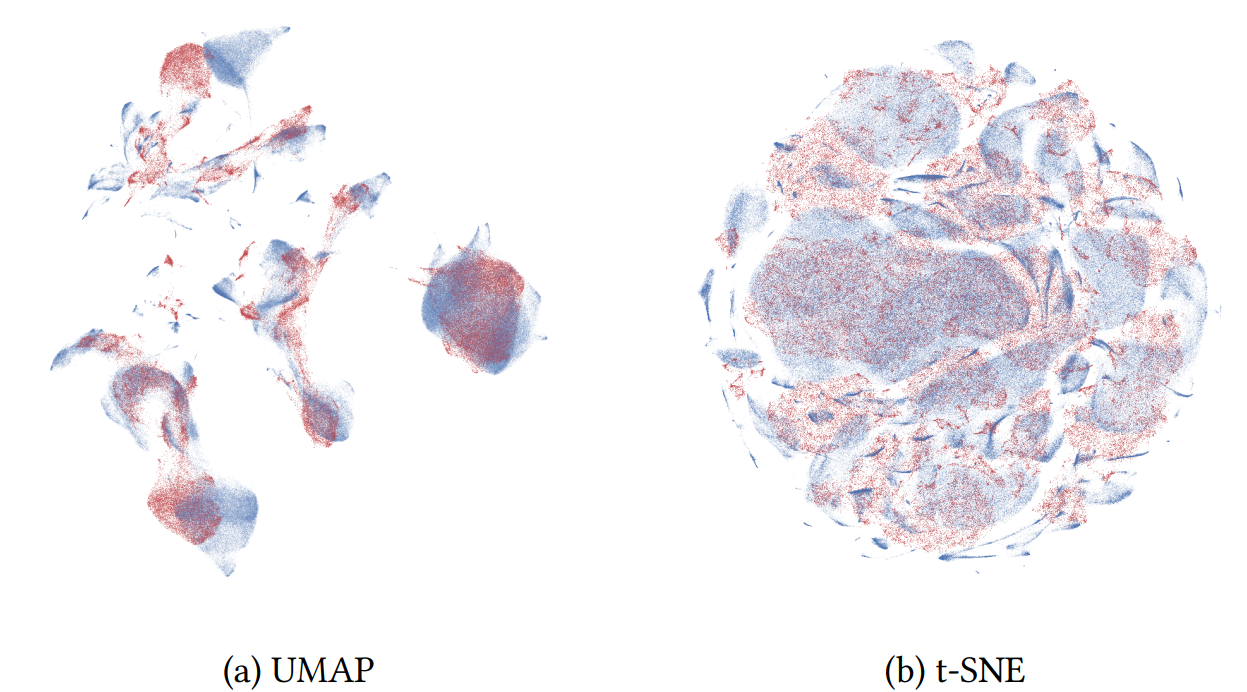
\includegraphics[width=0.8\textwidth]{images/umap.png}
    \caption{
    Procrustes-based alignment comparison of UMAP (left) and t-SNE (right) embeddings on flow cytometry data. Red points represent a 10\% subsample, blue points represent the full dataset \cite{mcinnes2020umapuniformmanifoldapproximation}.}
    \label{fig:umap_tsne_stability}
\end{figure}

One of UMAP's most significant advantages lies in its computational efficiency and scalability. Empirical evaluations demonstrate that UMAP is approximately an order of magnitude faster than t-SNE while maintaining comparable or superior visualization quality. The algorithm exhibits superior scaling performance across multiple dimensions: it scales efficiently with the number of data points, performs exceptionally well with high ambient dimensionality, and maintains computational efficiency when generating embeddings into dimensions higher than two. Unlike t-SNE, which requires global normalization and space trees that scale exponentially with embedding dimension, UMAP represents data as a fuzzy topological structure, allowing it to work without such computationally expensive constructs.

The algorithm's ability to preserve both local and global structure makes it particularly well-suited for interactive visualization applications in eXplainable AI. UMAP successfully maintains local cluster structures that facilitate identification of similar instances in synthetic neighborhoods, while simultaneously preserving global relationships that help users understand the overall data distribution and inter-cluster relationships \cite{becht2019evaluation}. 

UMAP's hyperparameters provide intuitive control over the embedding characteristics. The \texttt{n\_neighbors} parameter controls the balance between local and global structure preservation, with lower values emphasizing local structure and higher values focusing on global relationships. The \texttt{min\_dist} parameter controls the minimum distance between points in the low-dimensional representation, affecting the tightness of clusters in the final embedding \cite{mcinnes2020umap}. These parameters allow users to fine-tune the visualization based on their specific analytical requirements and the characteristics of the synthetic neighborhood being explored.

For 
synthetic
% $\text{LORE}_{sa}$'s 
neighborhood visualization requirements, UMAP's combination of theoretical rigor, computational efficiency, structure preservation, and stability makes it an ideal choice for projecting high-dimensional synthetic neighborhoods into interpretable 2D representations that facilitate effective human-AI interaction and explanation understanding.

\subsubsection{Comparative Analysis of Dimensionality Reduction Techniques}
Recent empirical research has provided comprehensive comparative evaluations of dimensionality reduction techniques across large-scale datasets, offering valuable insights for their application in eXplainable AI systems. Yang et al.\cite{yang2021dimensionality} conducted a systematic comparison of the four dimensionality reduction methods previously discussed: UMAP, t-SNE, PCA, and MDS, across 71 bulk transcriptomic datasets, evaluating their performance through both quantitative metrics and qualitative biological interpretability. This comparative analysis provides crucial evidence for selecting appropriate dimensionality reduction techniques.

The comprehensive evaluation framework uses quantitative metrics including \textbf{clustering accuracy} measured through Normalized Mutual Information (NMI) and Adjusted Rand Index (ARI), \textbf{neighborhood preservation} assessed via Jaccard index, and \textbf{computational efficiency} across varying dataset sizes \cite{yang2021dimensionality}.. 
As shown in Figure \ref{fig:DRcomparison1}, UMAP identified clustering structures in 41 out of 71 datasets (58\%), outperforming both t-SNE (37/71, 52\%), MDS (13/71, 18\%) and PCA (11/71, 15\%).

\begin{figure}
    \centering
    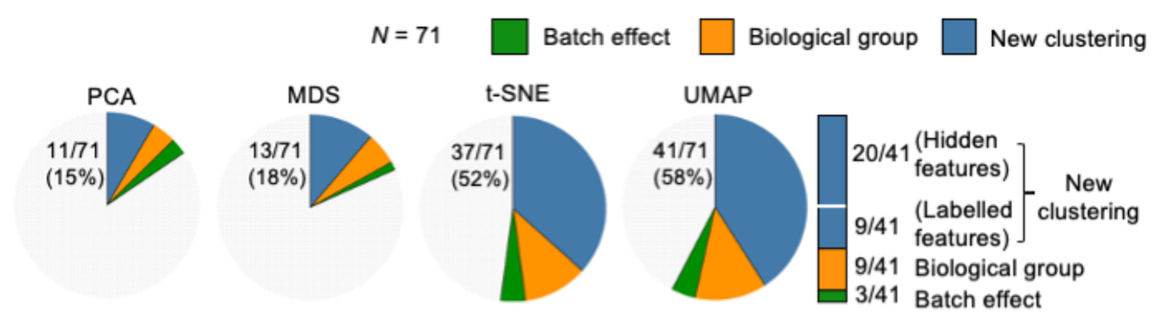
\includegraphics[width=\linewidth]{images/DRcomparison1.png}
    \caption{Dimensionality reduction techniques comparison results.}
    \label{fig:DRcomparison1}
\end{figure}

\paragraph{UMAP vs t-SNE}
The comparison between UMAP and t-SNE reveals complementary strengths, with UMAP demonstrating superior overall performance in large-scale data analysis. Both methods excel at preserving local neighborhood structures, with UMAP achieving an average neighborhood preservation score of 0.35 ± 0.091 compared to t-SNE's 0.36 ± 0.095, indicating comparable local structure retention capabilities \cite{yang2021dimensionality}. As shown in Figure \ref{fig:DRcomparison2}, both techniques substantially outperform linear methods in maintaining local relationships within high-dimensional data.

\begin{figure}
    \centering
    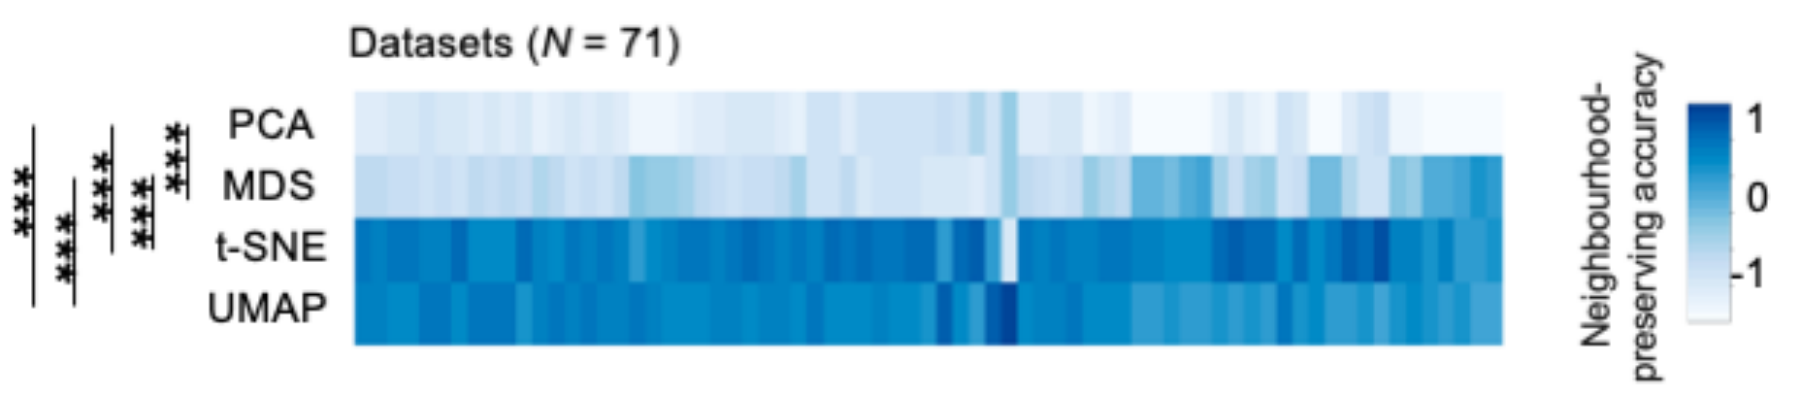
\includegraphics[width=\linewidth]{images/DRcomparison2.png}
    \caption{Dimensionality reduction techniques comparison results on neighborhood-preservation accuracy metric.}
    \label{fig:DRcomparison2}
\end{figure}

However, UMAP demonstrates superior clustering accuracy across multiple evaluation criteria. Figure \ref{fig:DRcomparison3} illustrates how UMAP consistently achieved the highest Normalized Mutual Information scores across five different clustering algorithms (k-means, hierarchical clustering, spectral clustering, Gaussian mixture model, and HDBSCAN), while t-SNE ranked second but with notably lower performance. 

\begin{figure}
    \centering
    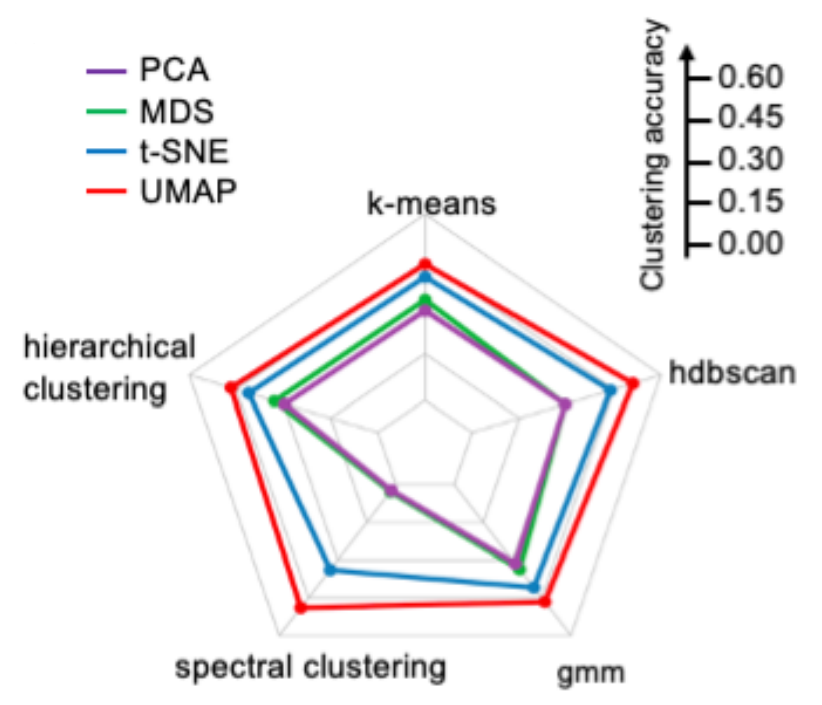
\includegraphics[width=0.7\linewidth]{images/DRcomparison3.png}
    \caption{Dimensionality reduction techniques comparison results on Normalized Mutual Information scores across five different clustering algorithms.}
    \label{fig:DRcomparison3}
\end{figure}

This enhanced clustering accuracy translates directly to improved separability of meaningful data structures, with UMAP achieving over 90\% random forest classification accuracy for batch effect detection compared to t-SNE's slightly lower performance.
A critical advantage of UMAP over t-SNE lies in computational efficiency, particularly for large-scale datasets. 
While both methods perform similarly for smaller datasets (200-500 samples), UMAP gains substantial advantages as dataset size increases. For datasets with 10,000 samples, UMAP requires approximately 3 minutes compared to t-SNE's 1.5 hours, representing more than a 25-fold improvement in computational speed. This efficiency advantage makes UMAP significantly more practical for interactive explanation systems that require responsive visualization updates.
Additionally, UMAP exhibits superior global structure preservation compared to t-SNE, arising from its use of Laplacian Eigenmap initialization and cross-entropy objective function rather than t-SNE's random initialization and KL-divergence approach \cite{yang2021dimensionality}. 

\paragraph{UMAP vs PCA}
The comparison between UMAP and PCA highlights fundamental differences between nonlinear manifold learning and linear dimensionality reduction approaches. While PCA demonstrates superior computational efficiency, processing 10,000 samples in approximately 20 seconds compared to UMAP's 3 minutes \cite{yang2021dimensionality}, UMAP provides dramatically superior performance in revealing complex data structures and meaningful clustering patterns.
The most striking difference appears in clustering structure identification capabilities. As demonstrated in Figure \ref{fig:DRcomparison1}, PCA identified clustering structures in only 11 out of 71 datasets (15\%), while UMAP revealed structures in 41 datasets (58\%). This improvement in structure detection capability is due to UMAP's ability to capture nonlinear relationships that PCA's linear transformation cannot represent effectively.
Clustering accuracy metrics reveal substantial performance differences between the methods. Figure \ref{fig:DRcomparison2} shows UMAP achieving consistently higher NMI scores across all clustering algorithms, while PCA demonstrated the poorest performance among all evaluated methods. This difference extends to neighborhood preservation, where UMAP's local structure retention (0.35 ± 0.091) significantly exceeds PCA's performance (0.19 ± 0.067), indicating that PCA's linear projections fail to maintain the local relationships crucial for interactive data exploration.
Despite PCA's computational advantages and interpretability through component loadings, its fundamental limitation lies in the linear assumption that proves inadequate for complex data structures. 

\paragraph{UMAP vs MDS}
The comparison between UMAP and MDS reveals the limitations of classical distance-preserving approaches when applied to complex high-dimensional data. MDS, while theoretically principled in its global distance preservation approach, demonstrates inferior performance across multiple evaluation criteria compared to UMAP's manifold learning methodology.
Computational efficiency represents a significant disadvantage for MDS. 
MDS as the slowest performing method across all dataset sizes, with particularly poor scaling characteristics that make it impractical for large-scale interactive applications. This computational burden severely limits MDS's applicability in explainability systems where responsive visualization updates are essential for effective human-AI interaction.
Clustering accuracy metrics reveal substantial performance gaps between the methods. UMAP consistently outperforms MDS across all clustering algorithms evaluated.
% , with MDS showing particularly poor performance in biological group separation tasks. 
The neighborhood preservation analysis highlights fundamental differences in the methods' design philosophies. While MDS focuses on preserving global pairwise distances, this emphasis comes at the expense of local neighborhood structure preservation. Figure \ref{fig:DRcomparison2} shows MDS achieving only moderate neighborhood preservation (0.26 ± 0.114) compared to UMAP's superior local structure retention (0.35 ± 0.091).
Structure identification capabilities further demonstrate UMAP's superiority. 
For 
% $\text{LORE}_{sa}$ 
synthetic
neighborhoods visualization applications, MDS's focus on global distance preservation may theoretically seem appealing for maintaining quantitative relationships within synthetic neighborhoods. However, the empirical evidence demonstrates that UMAP's superior local structure preservation, computational efficiency, and clustering accuracy make it significantly more suitable for interactive explanation systems where users need to explore and understand complex data relationships efficiently.

Figure \ref{fig:Dimensionality reduction webapp example} illustrates the comparison of the 4 methods on the same generated neighborhood of 3000 samples.

\begin{figure}[!ph]
    \centering

    \begin{subfigure}[c]{0.48\linewidth}
        \centering
        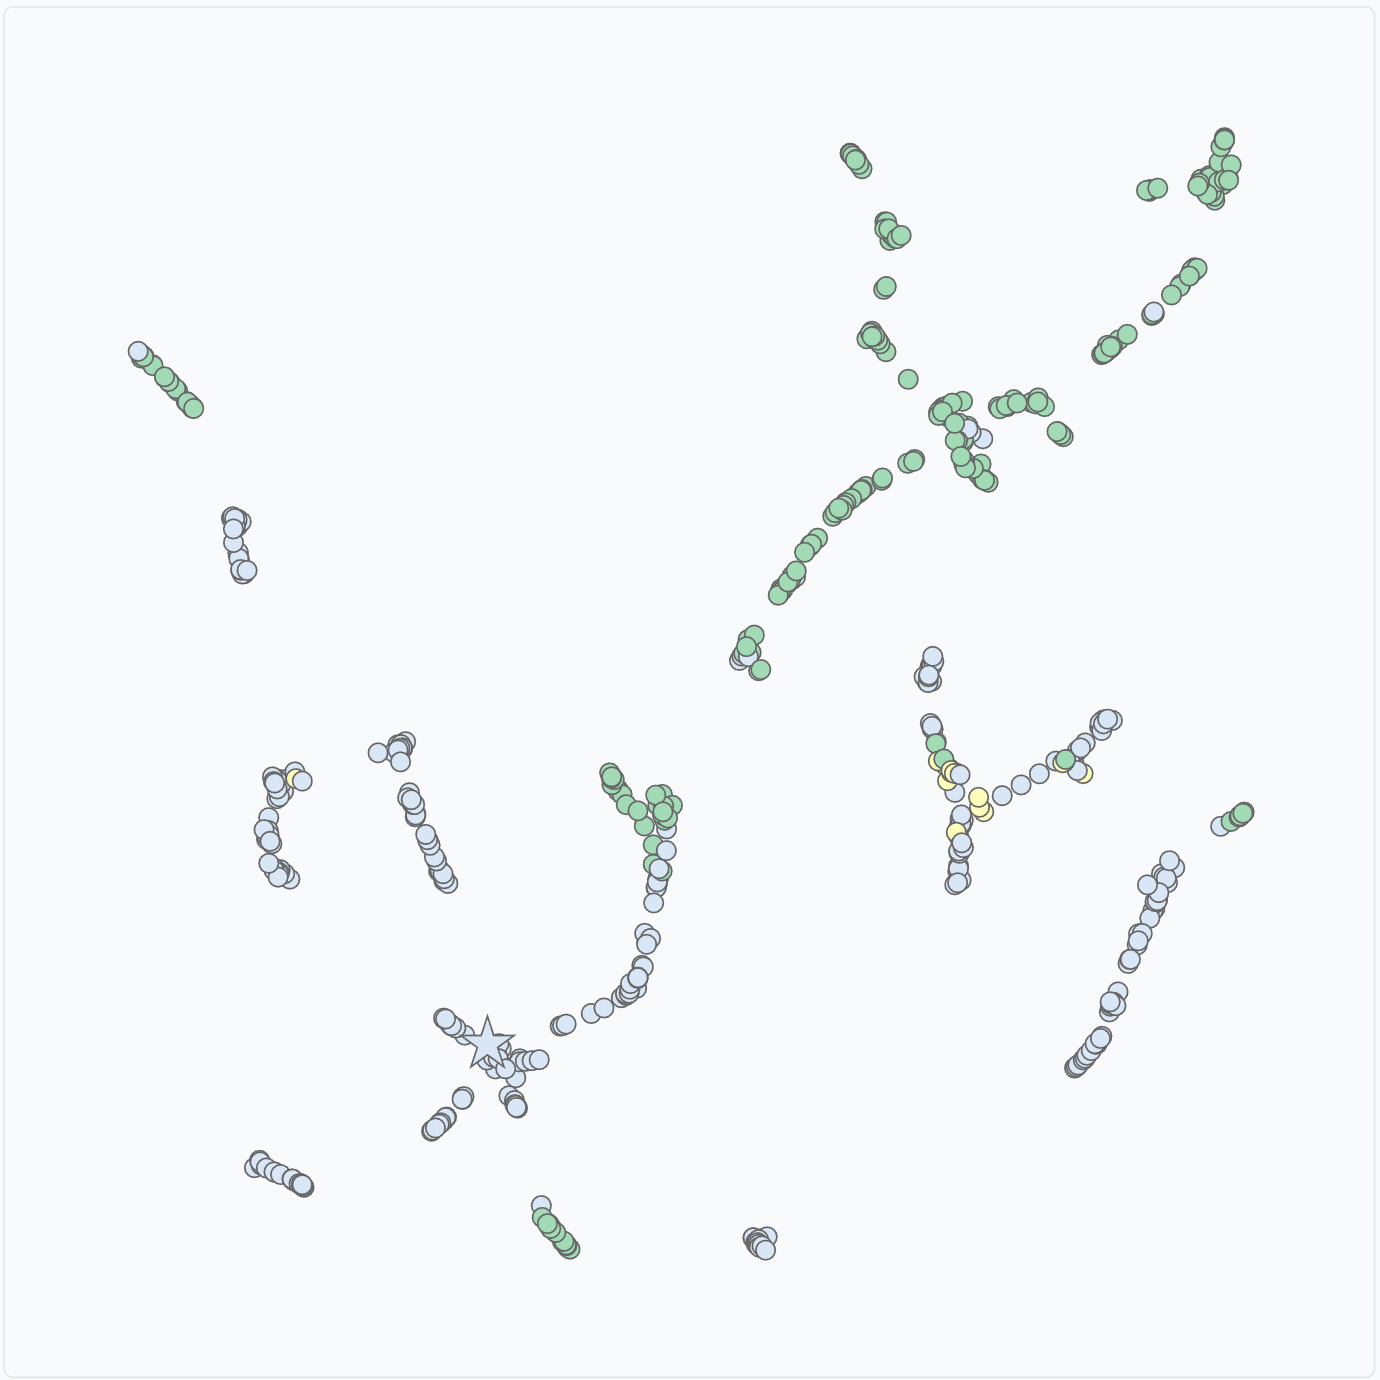
\includegraphics[width=\linewidth]{images/DR example UMAP.png}
        \caption{Uniform Manifold Approximation and Projection for dimension reduction}
        \label{fig:DR example UMAP}
    \end{subfigure}
    \hfill
    \begin{subfigure}[c]{0.48\linewidth}
        \centering
        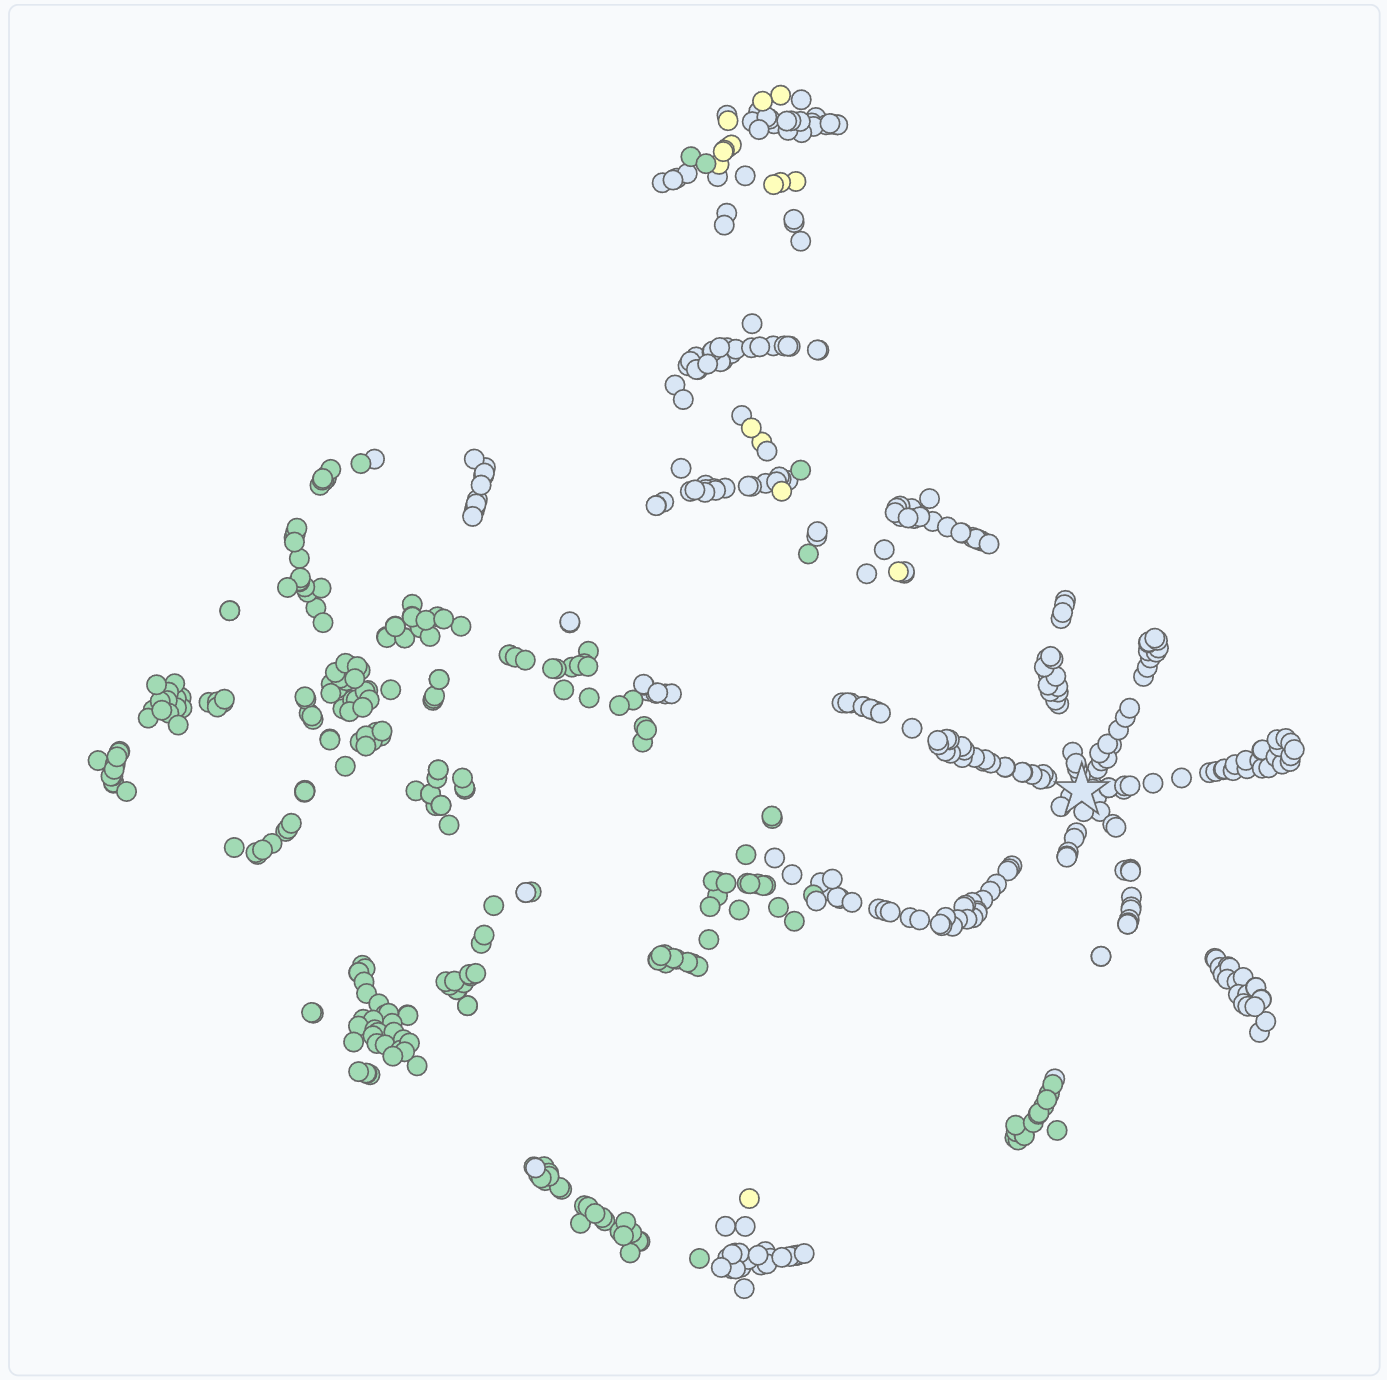
\includegraphics[width=\linewidth]{images/DR example t-sne.png}
        \caption{t-distributed Stochastic Neighbor Embedding}
        \label{fig:DR example t-SNE}
    \end{subfigure}
    
    \vspace{0.1cm} 

    \begin{subfigure}[c]{0.48\linewidth}
        \centering
        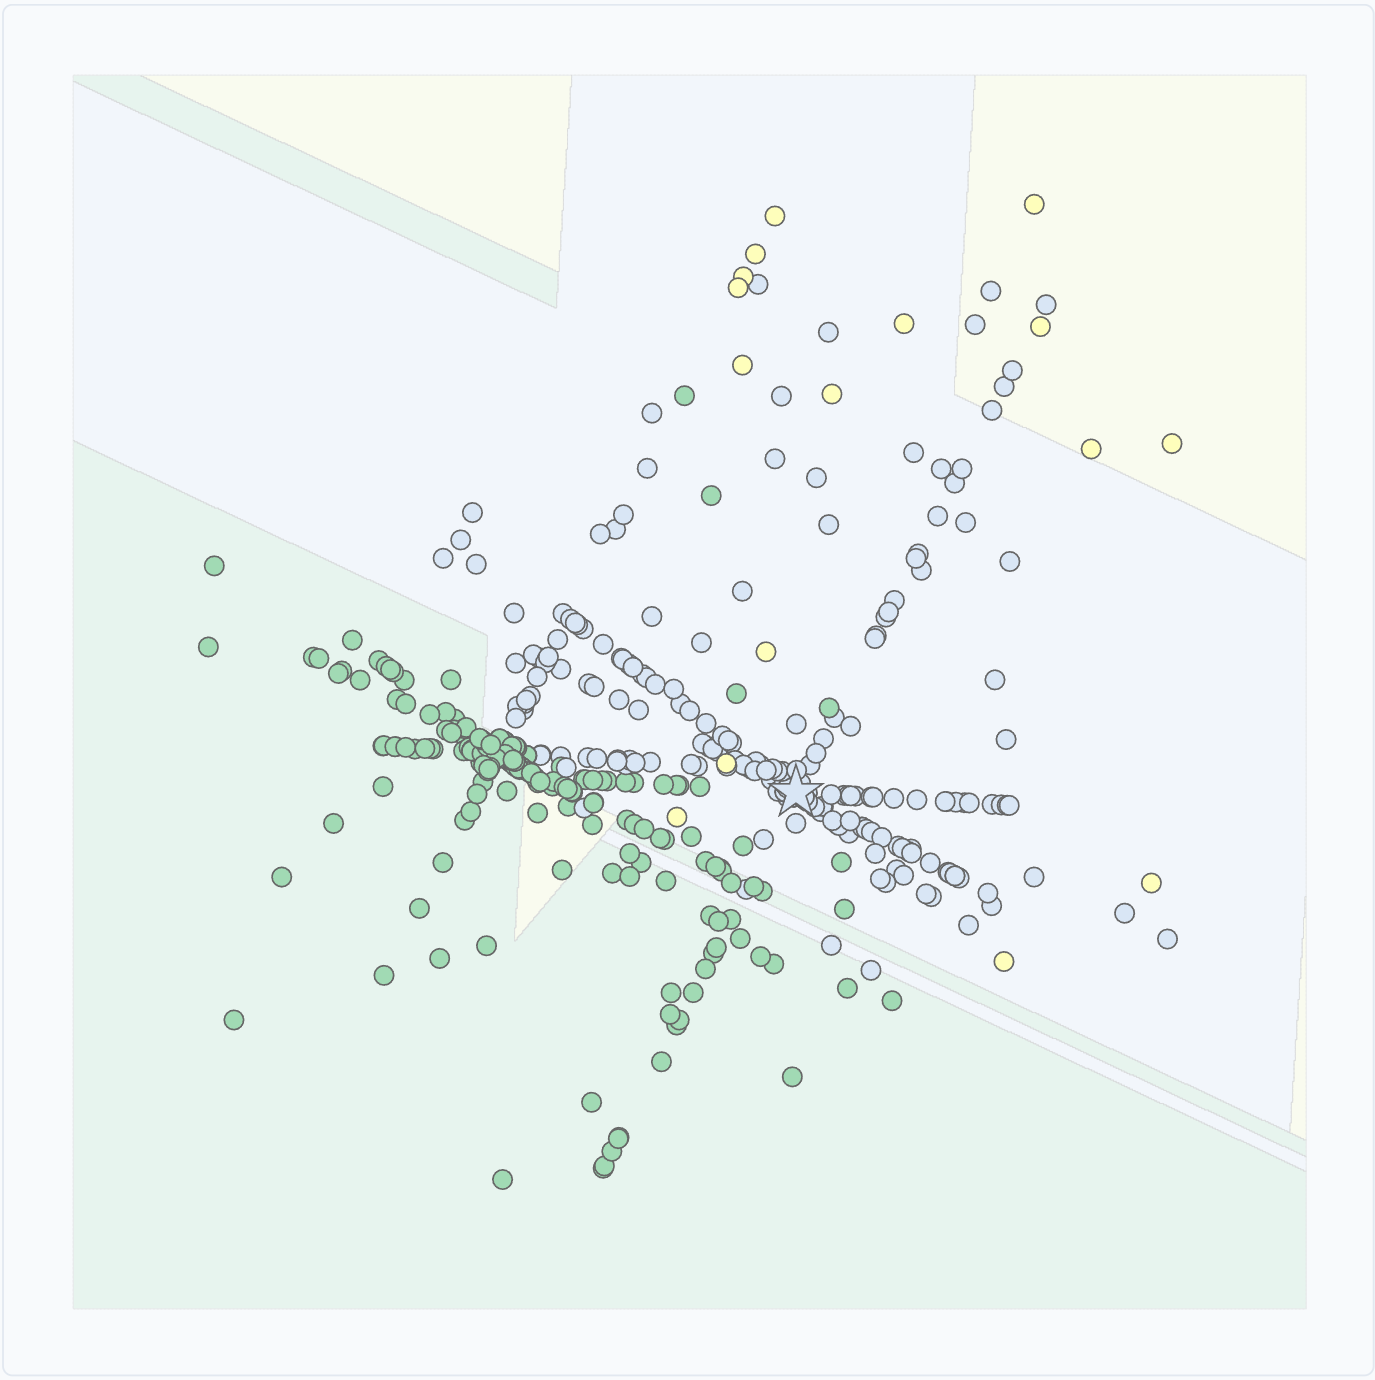
\includegraphics[width=\linewidth]{images/DR example PCA.png}
        \caption{Principal Component Analysis}
        \label{fig:DR example PCA}
    \end{subfigure}
    \hfill
    \begin{subfigure}[c]{0.48\linewidth}
        \centering
        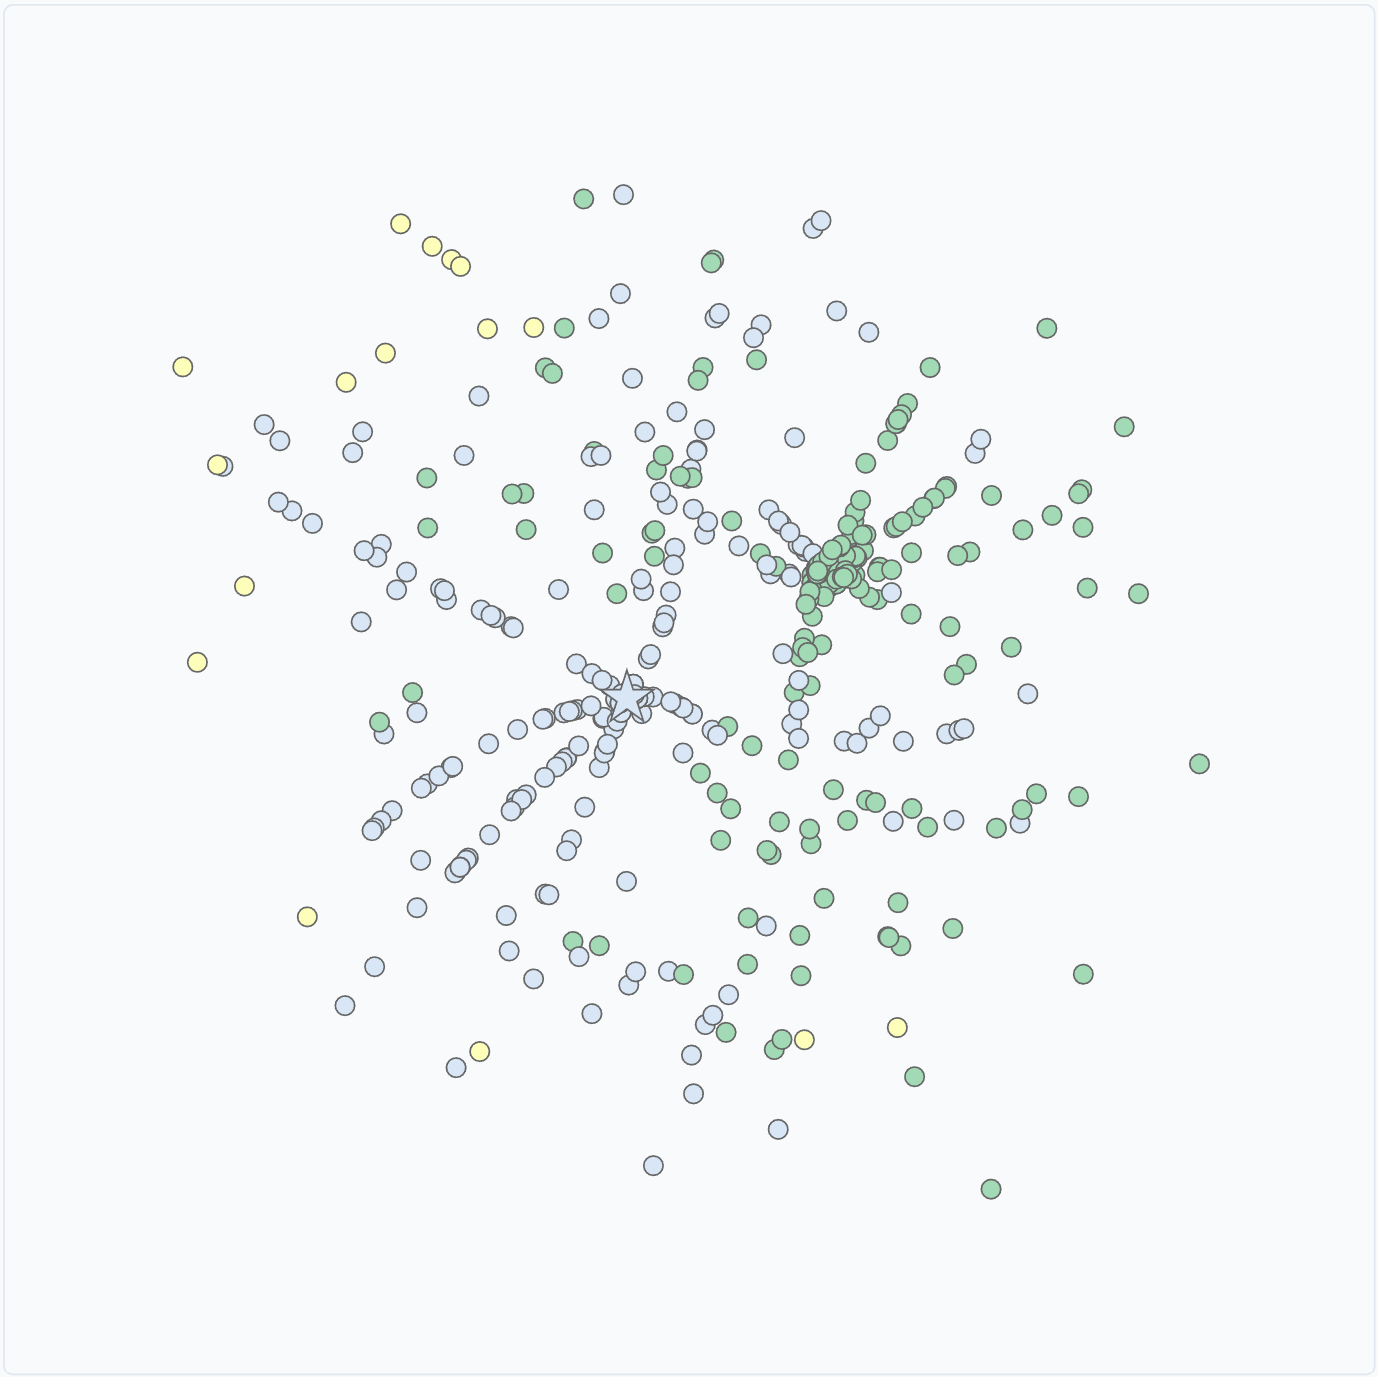
\includegraphics[width=\linewidth]{images/DR example MDS.png}
        \caption{MultiDimensional Scaling}
        \label{fig:DR example MDS}
    \end{subfigure}
    
    \caption{Example of the four dimensionality reduction techniques on a $\text{LORE}_{sa}$ generated neighborhood of 3000 samples, generated starting from the mean instance of the IRIS dataset}
    \label{fig:Dimensionality reduction webapp example}
\end{figure}